\begin{frame}[t]{Модел на Hodgkin-Huxley}
  Вече казахме, че липидната част на мембраната действа като кондензатор с капацитет $C$. 
  Помпите може да разглеждаме като проводници със съответна проводимост $g_{Na}$ и $g_{K}$.
  Проводимостта е обратнопропорционална на съпротивлението, 
  т.е. все едно това са резистори със съпротивления $\frac{1}{g_{Na}}$, $\frac{1}{g_{K}}$.
  Може да направим усложнение - $g_{l}$ проводимост на изтичащи йони от каналите. 
\end{frame}

\begin{frame}[t]{Модел на Hodgkin-Huxley}
  \begin{figure}[htbp!]
      \centering
      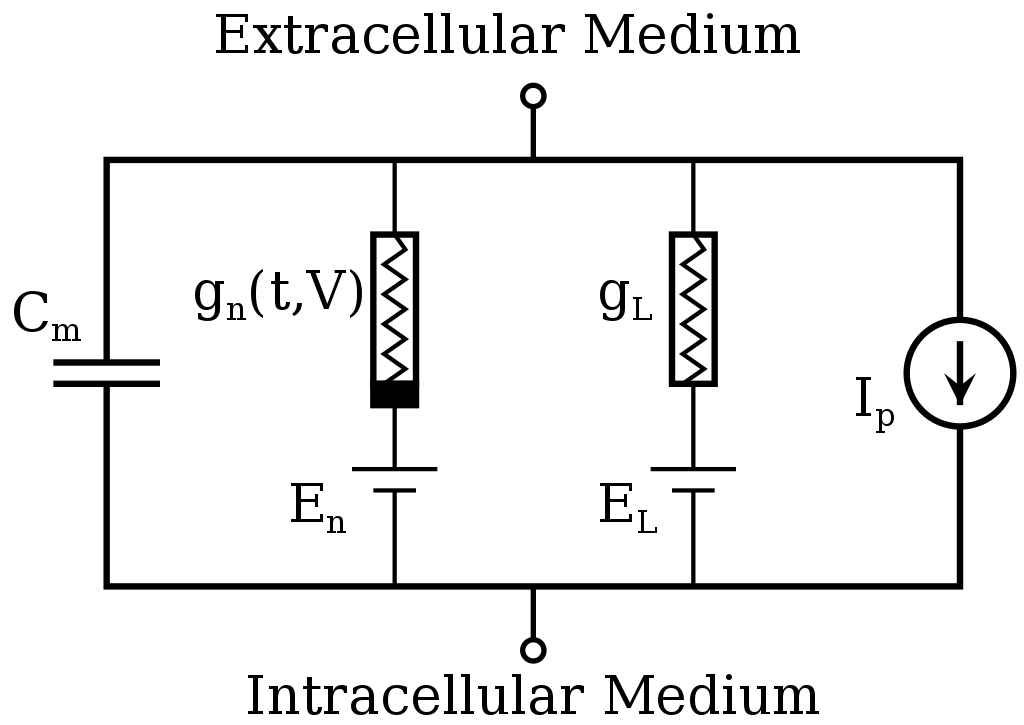
\includegraphics[width=\textwidth,height=0.7\textheight,keepaspectratio]{hodgkin-huxley-circuit.png}
      \caption{Еквивалентна електрическа верига от Wikipedia}
  \end{figure}
\end{frame}

\begin{frame}[t]{Модел на Hodgkin-Huxley}
  Да припомним, че $I = \dv{q}{t}$. 
  Сега може да изразим по дефиниция $C$ чрез моментните заряд $q$ и мембранния потенциал $V_m$, т.е. $C = \frac{q}{V}$.
  Откъдето $q = C V$ и $I_C = \dv{C V_m}{t} = \dv{C}{t}V_m + C\dv{V_m}{t}$. 
  Допускаме, че капацитета на мембраната не се променя с времето и достигаме до $I_C = C\dv{V}{t}$.
  Общия ток е сумата от 4-те тока, т.е.:
  \begin{equation*}
    I=C_{m}\dv{V_m}{t}+g_{K}(V_{m}-V_{K})+g_{Na}(V_{m}-V_{Na})+g_{l}(V_{m}-V_{l})
  \end{equation*}
\end{frame}

\begin{frame}[t]{Модел на Hodgkin-Huxley}
  От експериментите си върху аксона на сепия, Hodgkin и Huxley достигнали до следните изрази за пропускливостите:
  \begin{align*}
    &g_{K}=\tilde{g}_{K}n^4,\quad &g_{Na}=\tilde{g}_{Na}m^3h \\
    &\dv{p}{t}=\alpha_p(V_m)(1-n)-\beta_p(V_m)p,\quad &p={n,m,h}
  \end{align*}
  Тук $\tilde{g}_{K}$ и $\tilde{g}_{Na}$ са съответните максимални стойности на пропускливостта.
  Фунцкиите $\alpha_p$ и $\beta_p$ са експериментално установени като: 
  \begin{align*}
    &\alpha_{n}(V_{m})={\frac{0.01(10-V)}{\exp\left({\frac{10-V}{10}}\right)-1}} &\beta_{n}(V_{m})=0.125\exp\left(-\frac{V}{80}\right)\\
    &\alpha_{m}(V_{m})={\frac{0.1(25-V)}{\exp\left({\frac{25-V}{10}}\right)-1}} &\beta_{m}(V_{m})=4\exp\left(-\frac{V}{18}\right)\\
    &\alpha_{h}(V_{m})=0.07\exp\left(-{\frac{V}{20}}\right) &\beta_{h}(V_{m})={\frac{1}{\exp\left({\frac{30-V}{10}}\right)+1}}  
  \end{align*}
  Тук $V = V_{equilibrium} - V_m$.
\end{frame}

\begin{frame}[t]{Модел на Hodgkin-Huxley}
  Нека $a$ е радиусът на аксона, $R$ съпротивлението на цитоплазмата, а $x$ е ос по дължината на аксона.
  Може да се покаже, че $I={\frac{a}{2R}}\pdv[2]{V}{x}$, чрез тъй нареченото кабелно уравнение.
  Така за $V$ получаваме ЧДУ от тип реакция-дифузия.
  Моделът може да се усложни и за повече на вид йони, но трябва емпирично да се намерят изрази за съответстващите им пропускливости.

  Смисълът на $n$ е, че определя до колко са отворени \ce{K+} каналите.
  Аналогично $m$ и $h$ действат като активатор/деактиватор на \ce{Na+} каналите.
\end{frame}

\begin{frame}[t]{Модел на Hodgkin-Huxley}
  \begin{figure}[htbp!]
      \centering
      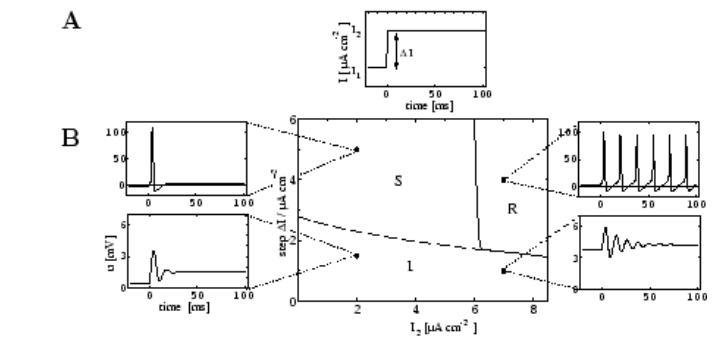
\includegraphics[width=\textwidth,height=0.7\textheight,keepaspectratio]{hodgkin-huxley-response.PNG}
      \caption{Подаване на стъпаловиден ток на модела на Hodgkin-Huxley, т.че $I_2$=$I_1$+$\Delta I$ \cite[Фиг 2.6]{Spiking}}
  \end{figure}
\end{frame}

\begin{frame}[t]{Модел на Hodgkin-Huxley}
  \begin{figure}[htbp!]
      \centering
      %\includemovie{1cm}{1cm}{hodgkin-huxley-graph.gif}
      %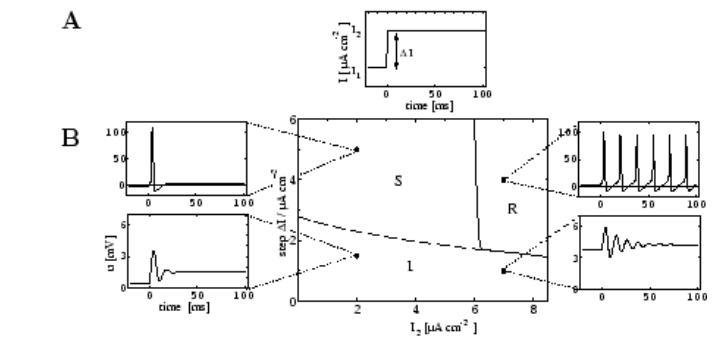
\includegraphics[width=\textwidth,height=0.7\textheight,keepaspectratio]{hodgkin-huxley-response.PNG}
      %\animategraphics{12}{hodgkin-huxley-graph/54223cdddc0944ffde281cbf29a5bf157wMigNej1EKKnEa6-}{0}{17}
      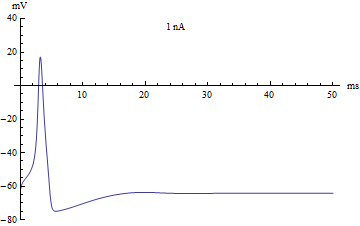
\includegraphics[width=\textwidth,height=0.7\textheight,keepaspectratio]{hodgkin-huxley-graph/54223cdddc0944ffde281cbf29a5bf157wMigNej1EKKnEa6-6.png}
      \caption{Симулация на модела на Hodgkin-Huxley от Wikipedia}
  \end{figure}
\end{frame}